% English, 15-minute seminar; edit this source in the existing document editor.
\documentclass[aspectratio=169,11pt]{beamer}
\usepackage[T1]{fontenc}
\usepackage{amsmath,amssymb,booktabs,array,graphicx}
\usetheme{Madrid}
\setbeamertemplate{navigation symbols}{}
\setbeamertemplate{itemize items}[circle]
\setbeamercolor{frametitle}{bg=blue!45!black}
\setbeamerfont{block title}{size=\small}
\setbeamersize{text margin left=6mm,text margin right=6mm}
\setlength{\tabcolsep}{4pt}
\graphicspath{{docs/presentations/figures/en/}}
\newcommand{\key}[1]{\textbf{\color{blue!55!black}#1}}
\newcommand{\flowfigure}[1]{\includegraphics[width=.97\textwidth,height=.62\textheight,keepaspectratio]{#1.pdf}}
\newcommand{\chartfigure}[1]{\includegraphics[width=.98\textwidth,height=.69\textheight,keepaspectratio]{#1.pdf}}
\title[Learning How Cities Respond]{Learning How Cities Respond}
\subtitle{Intervention-Conditioned Urban Representations\\[.6em]\small Dynamic responses to rail station openings}
\author{}\institute{}\date{}
\begin{document}
\section{Introduction}
\begin{frame}[plain]\titlepage\end{frame}

\begin{frame}{Why do places respond differently?}
\small
\begin{itemize}
 \item Rail expansion and transit-oriented development (TOD) connect station openings with land use, businesses and population change.
 \item Access, price capitalization and agglomeration vary with network position, land supply and local demand.
 \item Richer urban data support dynamic comparisons across places and outcomes.
\end{itemize}
\begin{block}{The planning question}
Can past station-opening responses help us compare potential responses in held-out cities?
\end{block}
\footnotesize Lu et al. (2016); Wang \& Xia (2024); Cervero \& Kockelman (1997);
Gonzalez-Navarro \& Turner (2018).
\end{frame}

\section{Related Work}

\begin{frame}{Related Work: transport effects and causal methods}
\small
\begin{itemize}
 \item \key{Transport effects}: rail access, firms, employment and population (Mayer \& Trevien, 2017); subways and urban growth (Gonzalez-Navarro \& Turner, 2018).
 \item \key{Space and timing}: housing and anticipation (Diao et al., 2017); neighborhood change and spillovers (Bardaka et al., 2018).
 \item \key{Counterfactuals}: matching (Imai et al., 2023), GSC (Xu, 2017), MC (Athey et al., 2021).
 \item \key{Dynamic identification}: staggered adoption and heterogeneity (Sun \& Abraham, 2021); pre-trends and sensitivity (Roth, 2022; Rambachan \& Roth, 2023).
\end{itemize}
\begin{block}{Our link}
Organize grid-level dynamic responses, method sources, support and diagnostics into traceable learning targets.
\end{block}
\end{frame}

\begin{frame}{Related Work: urban representations and response learning}
\small
\begin{tabular}{p{.24\textwidth}p{.67\textwidth}}
\toprule
Research area & Examples and focus\\
\midrule
Urban representations & Urban2Vec: street views and POIs; RegionDCL: buildings and POIs\\
Cross-city transfer & FLORAL: multimodal knowledge for data-limited cities\\
Causal urban learning & Weather2vec: spatial confounding; CauOD: flow prediction; CGNet-PIE: planning intervention effects\\
\bottomrule
\end{tabular}
\begin{block}{Response supervision}
Pre-treatment features enter the encoder. Estimated opening responses define the target.
We test response retrieval and prediction in held-out cities.
\end{block}
\footnotesize Wang et al. (2020); Li et al. (2023); Wei et al. (2016);
Tec et al. (2023); Zeng et al. (2022); Fang et al. (2025).
\end{frame}

\section{Problem and Data}

\begin{frame}{Problem setup: inputs, targets and tasks}
\small
\begin{block}{Each grid-level opening event}
Pre-treatment features $x_i$; frozen response signature $r_i$; observation mask $m_i$.
Learn $f:x_i\mapsto e_i$ and evaluate in held-out cities.
\end{block}
\begin{tabular}{p{.24\textwidth}p{.43\textwidth}p{.24\textwidth}}
\toprule
Task & Question & Metric\\
\midrule
Shape retrieval (main) & Do embedding neighbors share response shapes? & $\mathrm{nn\_corr@5}$\\
Magnitude prediction & How much response value can we recover? & RMSE\\
Direction prediction & Can we predict the response sign? & Sign accuracy\\
\bottomrule
\end{tabular}
\par\medskip\footnotesize Causal analysis covers housing, VIIRS, POI and population.
Current learning experiments use VIIRS and POI; masks and support define valid comparisons.
\end{frame}

\begin{frame}{Data: station openings across 44 cities}
\centering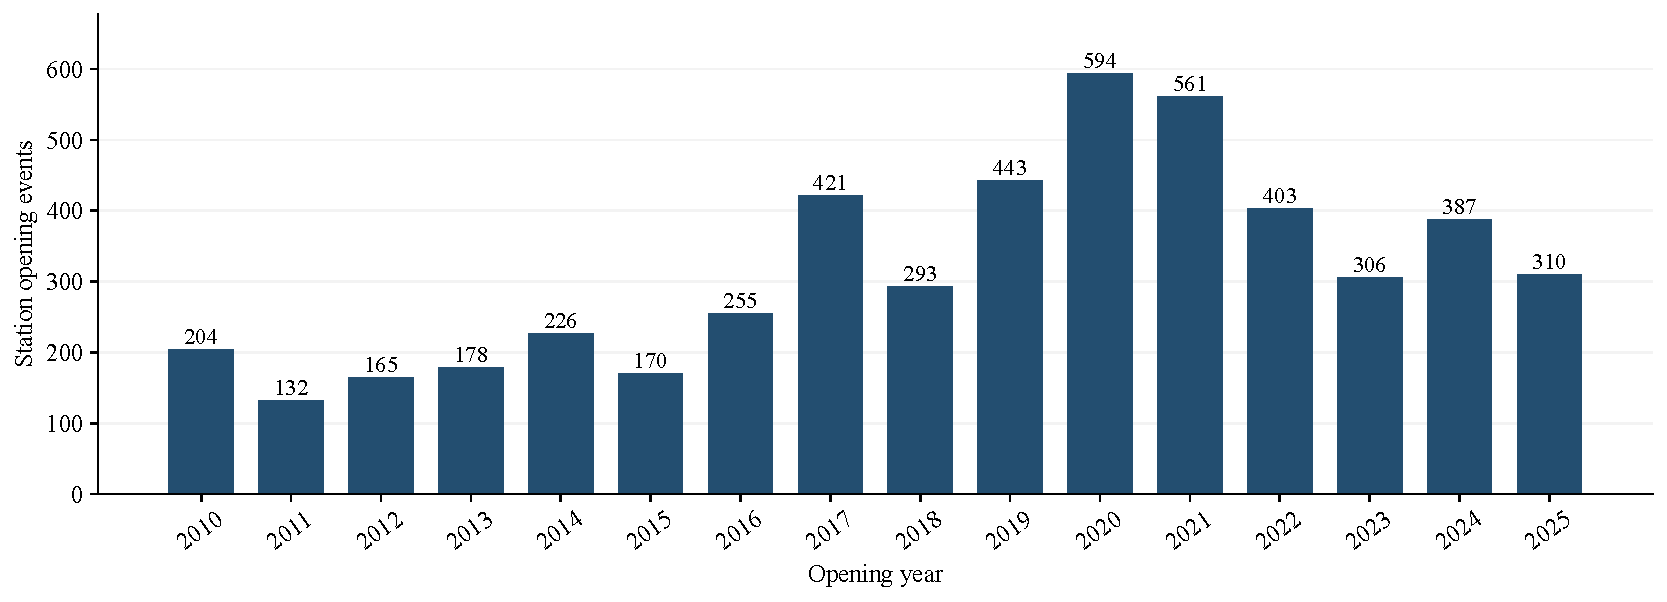
\includegraphics[width=.98\textwidth,height=.47\textheight,keepaspectratio]{intro_sample_years.pdf}
\par\raggedright\small
\begin{itemize}
 \item 5{,}048 events in 2010--2025; fixed $500\,\mathrm m\times500\,\mathrm m$ grids.
 \item VIIRS: 6 horizons, 1--24 months; POI: 4 outcomes $\times$ 3 years.
 \item Inputs: annual housing, POI, lights, population and Sentinel-2 features; 1--3 year lags.
\end{itemize}
\footnotesize Eligible labels depend on coverage and design support. Preprocessing uses training-side cities.
\end{frame}

\section{Causal Methods}

\begin{frame}{Causal labels: method routing and a frozen dataset}
\centering\flowfigure{intro_routing}
\par\raggedright\footnotesize Each grid and outcome family uses one assigned estimator.
Method panels describe their own supported samples. Responses, masks, method sources and diagnostics are frozen together.
\end{frame}

\begin{frame}{Matching: a grid-level difference-in-differences label}
\[
r^{\mathrm{match}}_{i,h}
=\big(Y^{\mathrm{post}}_{i,h}-\overline Y^{\mathrm{pre}}_i\big)
-\big(Y^{\mathrm{post}}_{c(i),h}-\overline Y^{\mathrm{pre}}_{c(i)}\big).
\]
\begin{itemize}
 \item $c(i)$ is the fixed matched control. Each grid receives its own response profile.
 \item Monthly baseline: months $-18$ to $-7$, leaving a six-month anticipation window.
 \item Annual baseline: the year before opening; post values follow outcome-specific horizon rules.
 \item Identification relies on comparable untreated trends and suitable controls; anticipation and spillovers shape design choices.
\end{itemize}
\footnotesize Imai et al. (2023). Grid labels and pooled event-study coefficients are distinct objects.
\end{frame}

\begin{frame}{GSC and MC: shared structure for counterfactuals}
\small
\begin{columns}[T]
\begin{column}{.48\textwidth}
\begin{block}{GSC: common factors}
\[
Y_{it}(0)=a_i+b_t+\ell_i^\top f_t+\varepsilon_{it}
\]
\begin{itemize}
 \item Untreated controls estimate time factors.
 \item Treated pre-periods estimate loadings and intercepts.
 \item Cross-validation selects rank; project the post-period counterfactual.
\end{itemize}
\end{block}
\end{column}
\begin{column}{.48\textwidth}
\begin{block}{MC: low-rank completion}
\[
\widehat Y_{it}(0)=\widehat a_i+\widehat b_t+\widehat L_{it}
\]
\begin{itemize}
 \item Fit observed untreated cells.
 \item A nuclear norm penalty controls the low-rank residual.
 \item Fill treated post-period counterfactuals.
\end{itemize}
\end{block}
\end{column}
\end{columns}
\par\medskip\key{Response}: $r_{i,h}=Y_{i,h}-\widehat Y_{i,h}(0)$.
Identification relies on stable shared structure and sufficient controls and pre-period support.
\par\footnotesize Xu (2017); Athey et al. (2021). GSC bootstrap and MC jackknife quantify model-conditional uncertainty.
\end{frame}

\begin{frame}{Event study: pooled dynamics and grid-level labels}
\[
Y_{ut}=a_u+b_t+
\sum_{h\ne-1}\beta_h T_u\,\mathbf 1\{t-E_{s(u)}=h\}+\varepsilon_{ut}.
\]
\begin{itemize}
 \item Unit and time fixed effects absorb stable differences and common changes.
 \item Matched controls use the treated event's clock $E_{s(u)}$; $h=-1$ is the zero reference.
 \item $\beta_h$ summarizes pooled dynamics; $r_{i,h}$ provides grid-level learning supervision.
 \item Released matching curves use TWFE. Staggered openings and heterogeneous effects shape its interpretation.
\end{itemize}
\footnotesize Sun \& Abraham (2021); Goodman-Bacon (2021). Heterogeneity-robust specifications are a further comparison.
\end{frame}

\section{Causal Evidence}

\begin{frame}{Pre-treatment diagnostics: evidence by method}
\centering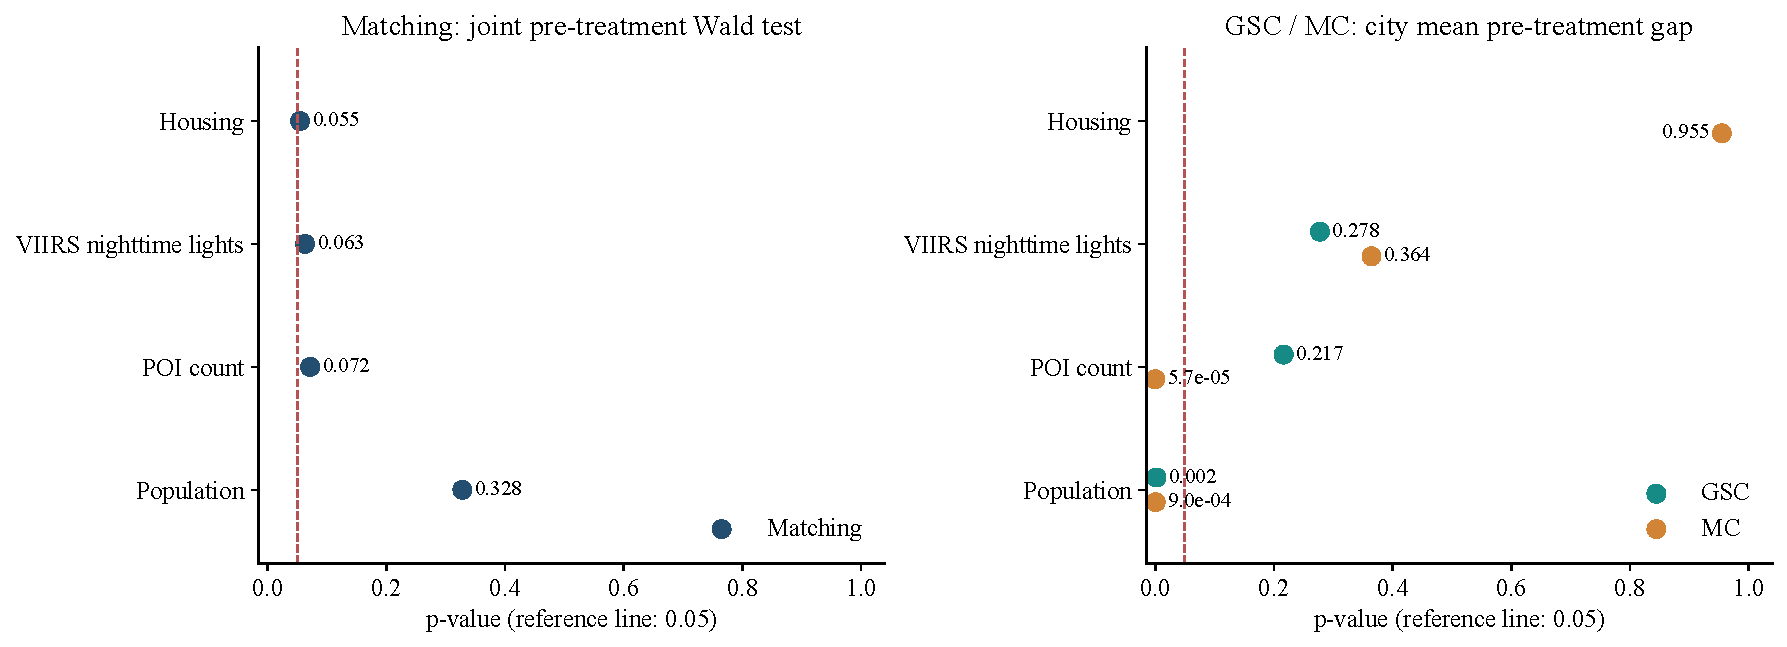
\includegraphics[width=.98\textwidth,height=.44\textheight,keepaspectratio]{intro_pretrend.pdf}
\par\raggedright
\begin{block}{Within-city controls; city-level inference; 5\% threshold}
\small
Matching retains the zero-pre-trend hypothesis for housing / VIIRS / POI count / population:
$p=0.055/0.063/0.072/0.328$.
GSC retains the zero-mean-gap hypothesis for VIIRS and POI count;
MC flags POI count, and GSC/MC flag population.
\end{block}
\footnotesize Matching: joint Wald; GSC/MC: city mean pre-gap test.
Housing, VIIRS and POI count matching reject at 10\%; grid-clustered tests also flag VIIRS and POI count.
MC housing/VIIRS cover 4/2 cities. Interpret tests alongside pre-fit and support.
\end{frame}

\begin{frame}{VIIRS: a sustained positive matched response}
\centering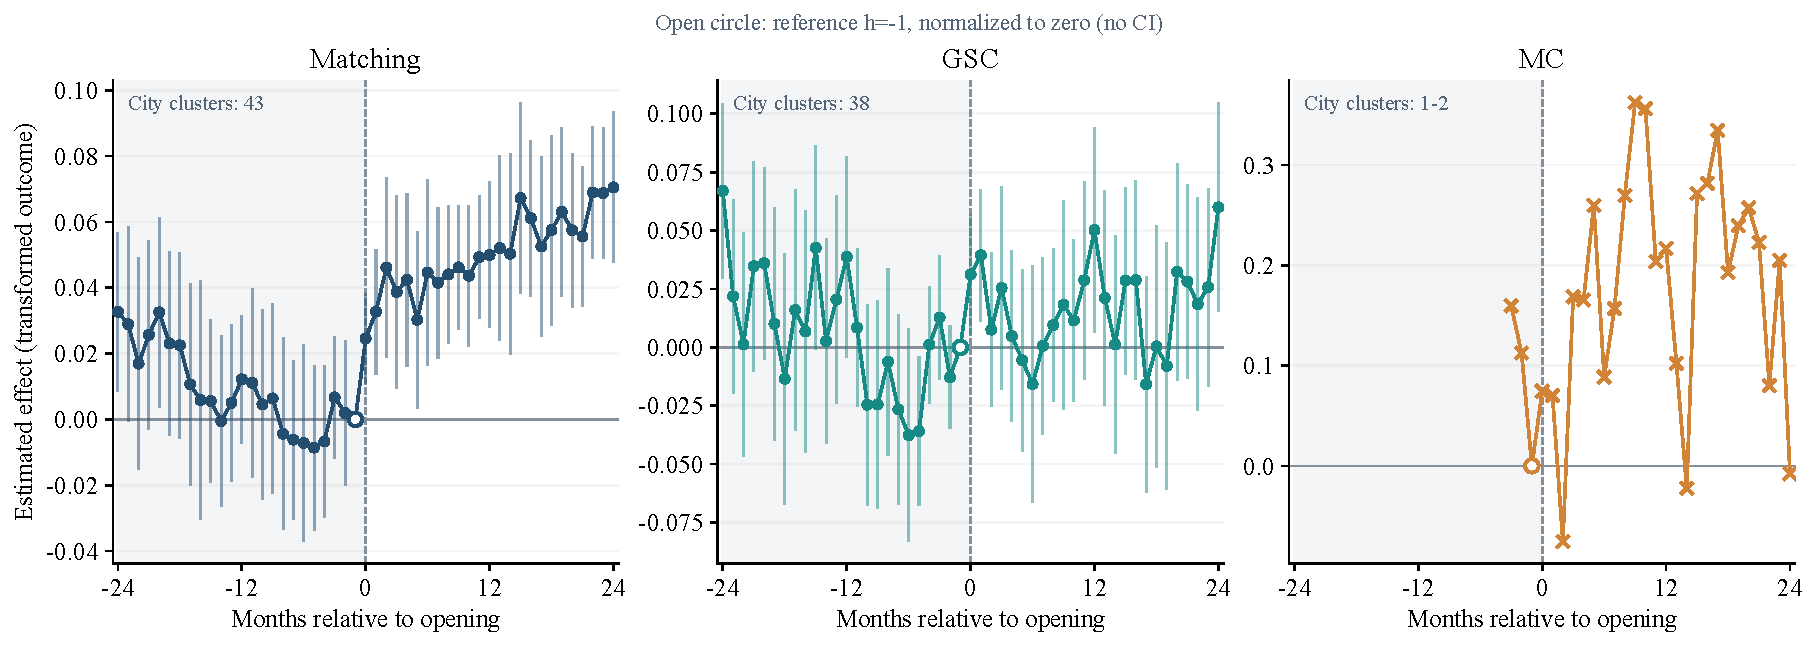
\includegraphics[width=.98\textwidth,height=.60\textheight,keepaspectratio]{intro_viirs_event_study.pdf}
\par\raggedright\footnotesize Within-city matching, 43 cities:
effects at 6/12/18/24 months are 0.0446/0.0500/0.0575/0.0705.
All four city-level 95\% CIs lie above zero; month 24: [0.0475, 0.0935]. Support: 2{,}255--2{,}264 units.
Asinh scale; panel axes and samples differ. Crosses mark estimates with fewer than 3 city clusters.
\end{frame}

\begin{frame}{POI count: positive activity responses after opening}
\centering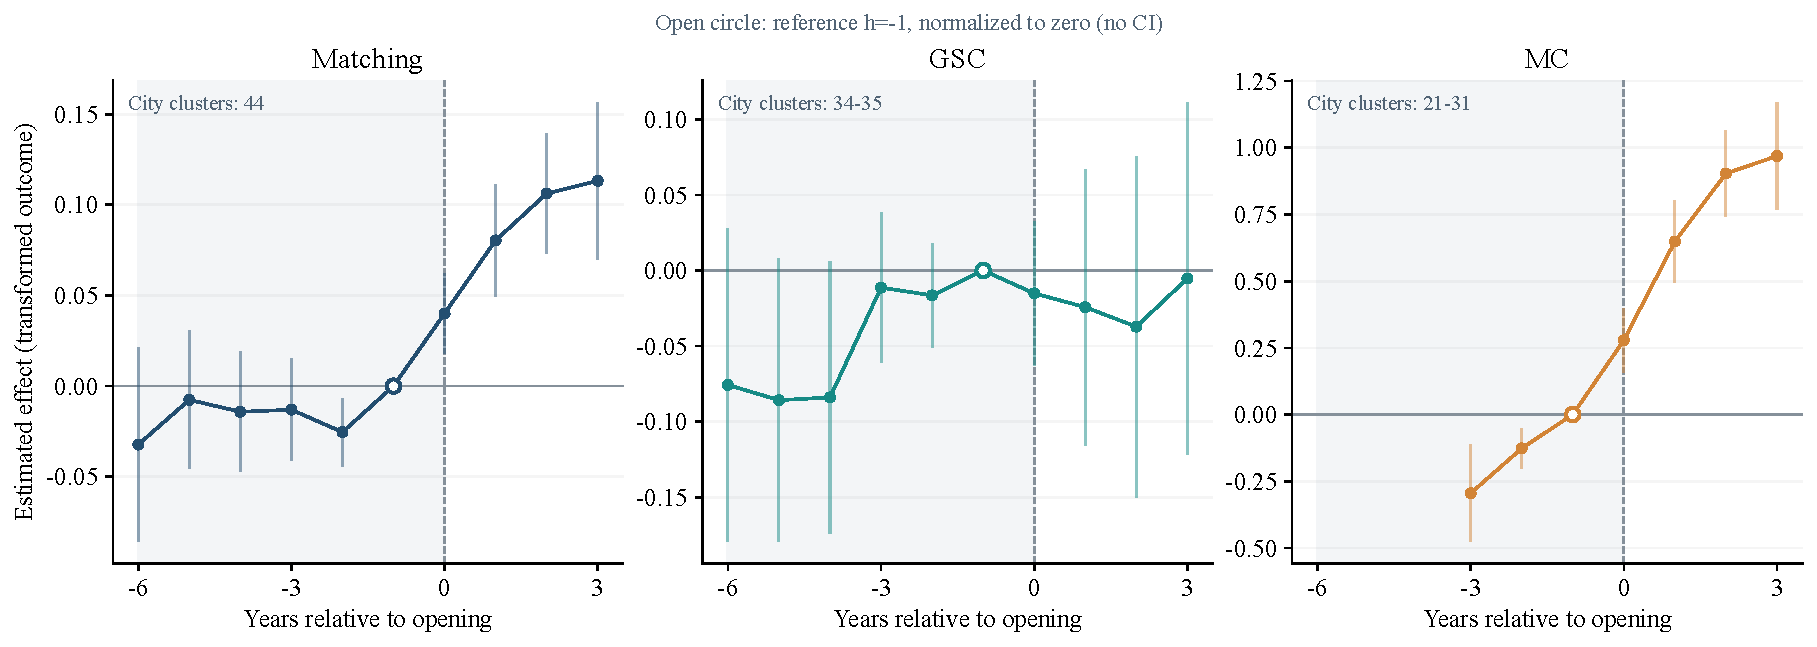
\includegraphics[width=.98\textwidth,height=.60\textheight,keepaspectratio]{intro_poi_event_study.pdf}
\par\raggedright\footnotesize Within-city matching, 44 cities:
effects in years 1/2/3 are 0.0803/0.1063/0.1132.
All three city-level 95\% CIs lie above zero; year 3: [0.0701, 0.1564]. Support: 2{,}476/2{,}242/1{,}947 units.
Log count scale; supported samples vary by method and horizon. POI count is an activity proxy.
\end{frame}

\section{Response Learning and Results}

\begin{frame}{Learning target: response shape and consistency}
\small
\[
s_{ij}=\operatorname{corr}_{w}(r_i,r_j)
\quad\text{on jointly observed cells within each family.}
\]
\begin{itemize}
 \item Average comparable family similarities. VIIRS has 6 cells; current POI pools 12 cells across 4 outcomes.
 \item Pearson captures shape; shifts and positive rescaling leave it unchanged. Evaluate magnitude and direction separately.
\end{itemize}
\medskip
\begin{tabular}{p{.49\textwidth}p{.20\textwidth}p{.20\textwidth}}
\toprule
Split-half consistency (SB corrected) & VIIRS & POI\\
\midrule
Matching / GSC & 0.806 / 0.887 & 0.285 / 0.156\\
\bottomrule
\end{tabular}
\par\medskip\noindent\key{Target evidence}: VIIRS has more consistent similarity structure; POI calls for outcome-level analysis.
\par\footnotesize Server diagnostic summary. Split consistency measures target structure; causal interpretation comes from design and diagnostics.
\end{frame}

\begin{frame}{Model: response supervision for pre-treatment features}
\centering\flowfigure{intro_model}
\par\raggedright\footnotesize Default: tabular MLP and a normalized 128-dimensional embedding.
Prediction heads read the embedding. Images, station/year conditioning and the FIFO queue are optional;
historical main comparisons use tabular inputs. The optional image branch uses frozen DINOv2.
\end{frame}

\begin{frame}{Joint objective: neighbors, similarity and response values}
\small
\begin{tabular}{p{.20\textwidth}p{.71\textwidth}}
\toprule
Loss & Role\\
\midrule
$L_{\rm align}$ & Fit embedding neighbor probabilities with positive response similarity as soft weights\\
$L_{\rm dist}$ & Fit numerical response similarity with embedding cosine similarity\\
$L_{\rm pred}$ & Recover response values with masks and label-weighted MSE\\
\bottomrule
\end{tabular}
\[
L_{\rm dist}=\operatorname{mean}_{(i,j)\in\mathcal V}
(e_i^\top e_j-\widetilde s_{ij})^2
\]
\[
\boxed{L=0.25L_{\rm align}+0.25L_{\rm dist}+0.50L_{\rm pred}}
\]
\key{Empirical question}: does joint supervision improve held-out city retrieval?
\par\footnotesize Default temperature $\tau=0.07$; $\mathcal V$ excludes self and invalid pairs.
$\widetilde s$ uses SE shrinkage when enabled. Constant within-grid weights cancel in Pearson but affect prediction.
\end{frame}

\begin{frame}{Evaluation: shape, magnitude and direction}
\small
\begin{tabular}{p{.21\textwidth}p{.36\textwidth}p{.34\textwidth}}
\toprule
Task & Metric & Baselines\\
\midrule
Shape retrieval & Mean response similarity of 5 neighbors & Raw features, appearance autoencoder, random neighbors\\
Magnitude prediction & RMSE & Training mean, ridge, kNN\\
Direction prediction & Sign accuracy & Training majority sign\\
\bottomrule
\end{tabular}
\begin{itemize}
 \item Direct controls: fixed 5-fold city CV, fold-specific preprocessing and inner tuning.
 \item Trained embeddings: earlier city split, 3 seeds and a shared candidate pool.
 \item Interpret each protocol separately; next, compare paired city-level gains under one CV protocol.
\end{itemize}
\footnotesize Main metric: $\mathrm{nn\_corr@5}$. Seed SD measures training variability; city-level intervals measure variation across cities.
\end{frame}

\begin{frame}{Result 1: features carry a held-out city response signal}
\centering\chartfigure{intro_city_controls}
\par\raggedright\footnotesize Server 5-fold city-CV summary.
Raw retrieval gains over random: 0.0424/0.0451 (VIIRS/POI).
Ridge RMSE: 0.3627/0.4442; direction gains over majority sign: 1.2/5.0 percentage points.
Each metric answers a separate question.
\end{frame}

\begin{frame}{Result 2: retrieval with trained embeddings}
\centering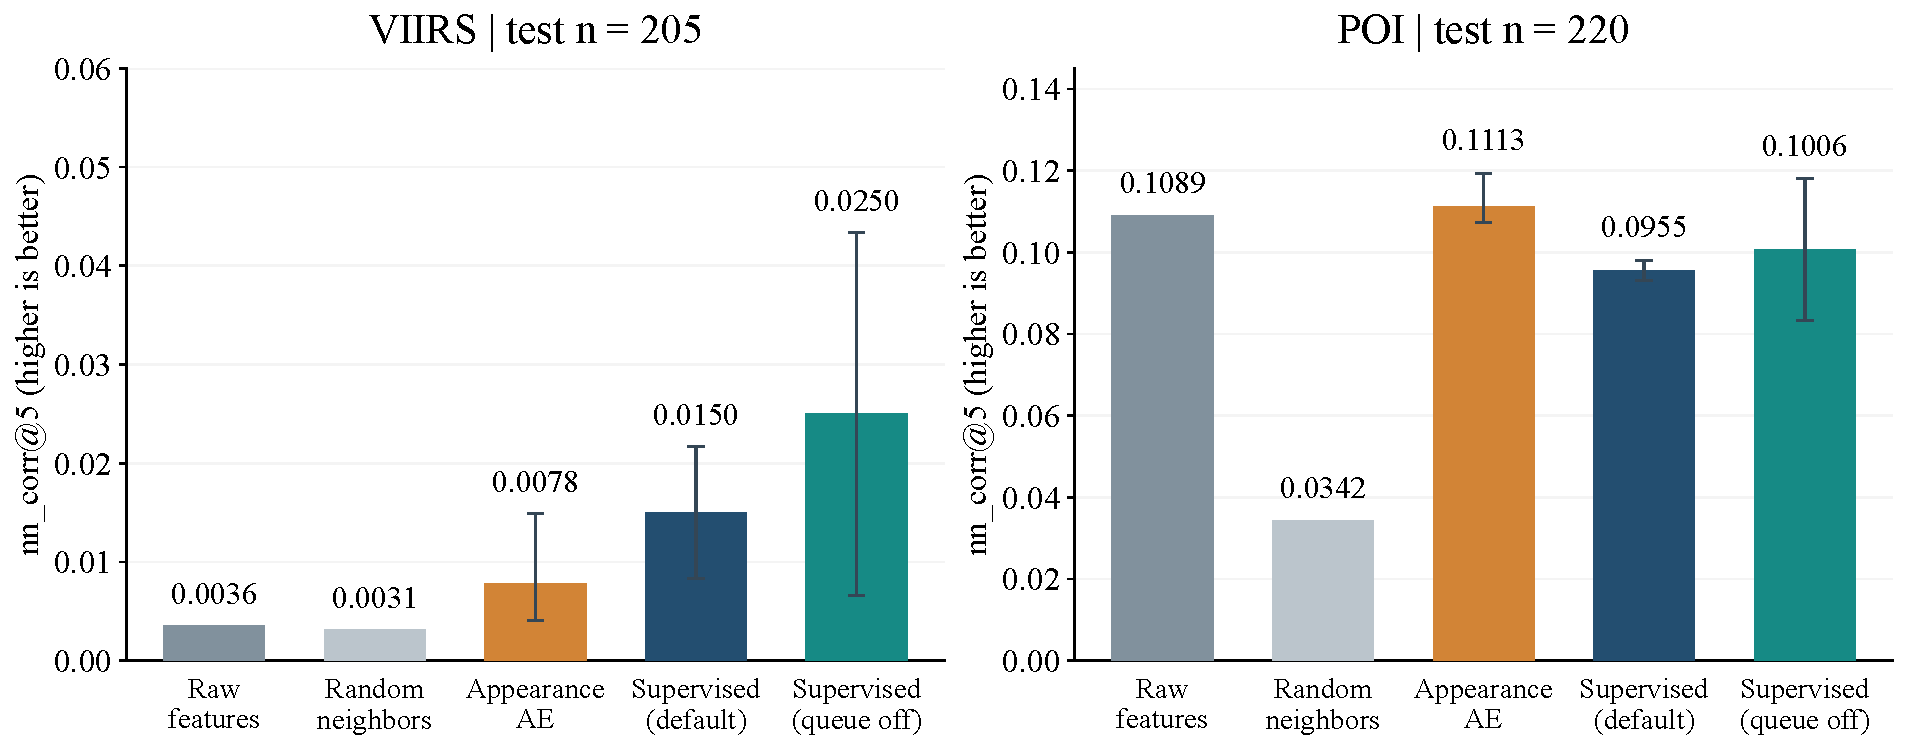
\includegraphics[width=.98\textwidth,height=.62\textheight,keepaspectratio]{intro_representation_benchmark.pdf}
\par\raggedright\footnotesize
VIIRS: default $0.0150\pm0.0067$, raw $0.0036$; mean gain $+0.0114$.
POI: default $0.0955\pm0.0025$, raw $0.1089$; mean gain $-0.0134$.
VIIRS shows an initial gain; POI favors raw geometry. Earlier test pools: 205/220.
Bars: reported scores. Error bars: 3-seed SD for supervised models; reported range for the appearance AE.
Panel y-scales differ; each starts at zero.
\end{frame}

\begin{frame}{Ablation: gains over raw feature retrieval}
\centering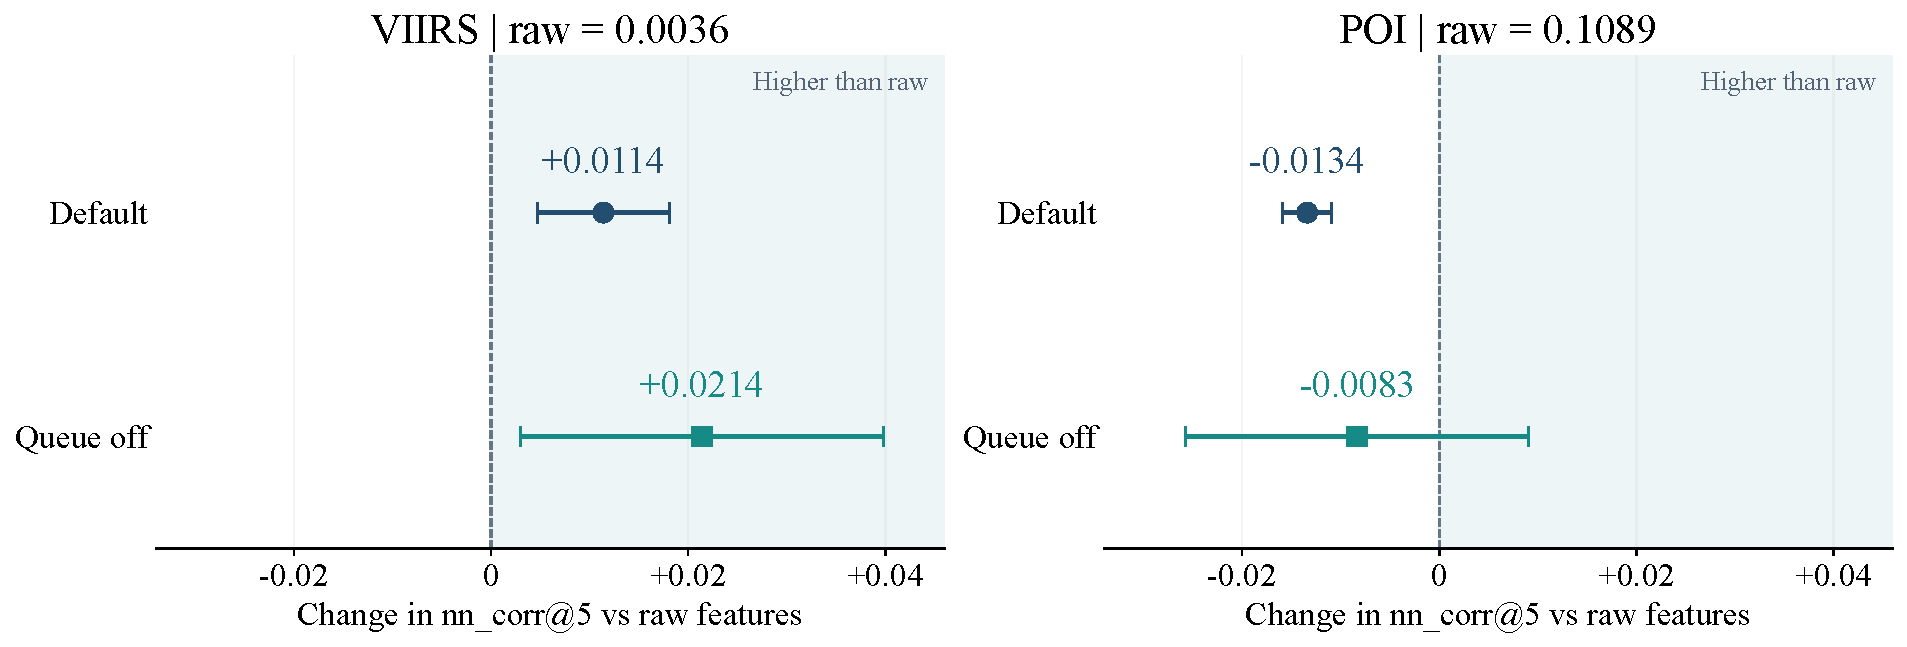
\includegraphics[width=.98\textwidth,height=.54\textheight,keepaspectratio]{intro_representation_gains.pdf}
\par\raggedright
\begin{block}{Initial gains depend on the response family}
\small VIIRS: default $+0.0114$, queue off $+0.0214$.
POI favors raw features. Queue removal raises the mean and increases seed variability.
\end{block}
\footnotesize Absolute correlation-score change on a shared x-scale.
Markers: 3-seed mean gains $\pm$ SD (training variability).
Earlier city split; zero is the fixed raw baseline.
\end{frame}

\section{Conclusion}

\begin{frame}{Takeaways: causal evidence and cross-city learning}
\small
\begin{itemize}
 \item \key{Causal evidence}: positive VIIRS and POI count dynamics in within-city matched samples.
 \item \key{Feature signal}: small held-out city prediction gains, with ridge as a direct baseline.
 \item \key{Trained embeddings}: an initial VIIRS retrieval gain; stronger raw geometry for POI.
\end{itemize}
\begin{block}{Next test: preserve raw geometry and add predicted responses}
\[
z_i(\lambda)=[\sqrt{1-\lambda}\,\bar x_i,\;\sqrt{\lambda}\,\bar h_i]
\]
Inner cities select the fusion weight; outer cities measure paired gains.
$\lambda=0$ recovers raw geometry on the shared support set.
\end{block}
\footnotesize Fusion evaluation is implemented; results are pending.
The goal is to turn traceable local responses into useful comparisons across cities.
\end{frame}

\section{References}
\begin{frame}[allowframebreaks]{References}
  \scriptsize
  \begin{thebibliography}{99}
    \setbeamertemplate{bibliography item}[text]
    \bibitem{abadie2003} Abadie, A., \& Gardeazabal, J. (2003). The economic costs of conflict: A case study of the Basque Country. American Economic Review.
    \bibitem{abadie2010} Abadie, A., Diamond, A., \& Hainmueller, J. (2010). Synthetic control methods for comparative case studies. Journal of the American Statistical Association.
    \bibitem{abadie2021} Abadie, A. (2021). Using synthetic controls: Feasibility, data requirements, and methodological aspects. Journal of Economic Literature.
    \bibitem{xu2017} Xu, Y. (2017). Generalized synthetic control method. Political Analysis.
    \bibitem{athey2021} Athey, S., Bayati, M., Doudchenko, N., Imbens, G., \& Khosravi, K. (2021). Matrix completion methods for causal panel data models. Journal of the American Statistical Association.
    \bibitem{callaway2021} Callaway, B., \& Sant'Anna, P. H. C. (2021). Difference-in-differences with multiple time periods. Journal of Econometrics.
    \bibitem{sun2021} Sun, L., \& Abraham, S. (2021). Estimating dynamic treatment effects in event studies with heterogeneous treatment effects. Journal of Econometrics.
    \bibitem{goodman2021} Goodman-Bacon, A. (2021). Difference-in-differences with variation in treatment timing. Journal of Econometrics.
    \bibitem{imai2023} Imai, K., Kim, I. S., \& Wang, E. H. (2023). Matching methods for causal inference with time-series cross-sectional data. American Journal of Political Science.
    \bibitem{roth2022} Roth, J. (2022). Pretest with caution: Event-study estimates after testing for parallel trends. American Economic Review: Insights.
    \bibitem{rambachan2023} Rambachan, A., \& Roth, J. (2023). A more credible approach to parallel trends. Review of Economic Studies.
    \bibitem{baum2000} Baum-Snow, N., \& Kahn, M. E. (2000). The effects of new public projects to expand urban rail transit. Journal of Public Economics.
    \bibitem{gibbons2005} Gibbons, S., \& Machin, S. (2005). Valuing rail access using transport innovations. Journal of Urban Economics.
    \bibitem{debrezion2007} Debrezion, G., Pels, E., \& Rietveld, P. (2007). The impact of railway stations on residential and commercial property value: A meta-analysis. The Journal of Real Estate Finance and Economics.
    \bibitem{zheng2008} Zheng, S., \& Kahn, M. E. (2008). Land and residential property markets in a booming economy: New evidence from Beijing. Journal of Urban Economics. \href{https://doi.org/10.1016/j.jue.2007.04.010}{[Source]}
    \bibitem{gonzalez2018} Gonzalez-Navarro, M., \& Turner, M. A. (2018). Subways and urban growth: Evidence from Earth. Journal of Urban Economics. \href{https://www.nber.org/papers/w24996}{[Source]}
    \bibitem{dong2017} Dong, H. (2017). Rail-transit-induced gentrification and the affordability paradox of TOD. Journal of Transport Geography.
    \bibitem{cervero1997} Cervero, R., \& Kockelman, K. (1997). Travel demand and the 3Ds: Density, diversity, and design. Transportation Research Part D.
    \bibitem{lu2016} Lu, K., Han, B., Lu, F., \& Wang, Z. (2016). Urban rail transit in China: Progress report and analysis (2008--2015). Urban Rail Transit. \href{https://doi.org/10.1007/s40864-016-0048-7}{[Source]}
    \bibitem{bao2018} Bao, X. (2018). Urban rail transit present situation and future development trends in China: Overall analysis based on national policies and strategic plans in 2016--2020. Urban Rail Transit. \href{https://doi.org/10.1007/s40864-018-0078-4}{[Source]}
    \bibitem{wang2024} Wang, L., \& Xia, H. (2024). A comprehensive review of the development characteristics and future trends of TOD in Chinese urban rail transit. Urban Rail Transit. \href{https://doi.org/10.1007/s40864-024-00228-2}{[Source]}
    \bibitem{jean2016} Jean, N., Burke, M., Xie, M., Davis, W. M., Lobell, D. B., \& Ermon, S. (2016). Combining satellite imagery and machine learning to predict poverty. Science.
    \bibitem{rolf2021} Rolf, E., Proctor, J., Carleton, T., Bolliger, I., Shankar, V., Ishihara, M., Recht, B., \& Hsiang, S. (2021). A generalizable and accessible approach to machine learning with global satellite imagery. Nature Communications.
    \bibitem{chen2020} Chen, T., Kornblith, S., Norouzi, M., \& Hinton, G. (2020). A simple framework for contrastive learning of visual representations. International Conference on Machine Learning.
    \bibitem{he2020} He, K., Fan, H., Wu, Y., Xie, S., \& Girshick, R. (2020). Momentum contrast for unsupervised visual representation learning. IEEE/CVF Conference on Computer Vision and Pattern Recognition.
    \bibitem{khosla2020} Khosla, P., Teterwak, P., Wang, C., Sarna, A., Tian, Y., Isola, P., Maschinot, A., Liu, C., \& Krishnan, D. (2020). Supervised contrastive learning. Advances in Neural Information Processing Systems.
    \bibitem{oquab2024} Oquab, M., Darcet, T., Moutakanni, T., et al. (2024). DINOv2: Learning robust visual features without supervision. Transactions on Machine Learning Research.
    \bibitem{scholkopf2021} Sch\"olkopf, B., Locatello, F., Bauer, S., Ke, N. R., Kalchbrenner, N., Goyal, A., \& Bengio, Y. (2021). Toward causal representation learning. Proceedings of the IEEE. \href{https://arxiv.org/abs/2102.11107}{[Source]}

    \bibitem{mayer2017} Mayer, T., \& Trevien, C. (2017). The impact of urban public transportation: Evidence from the Paris region. Journal of Urban Economics. \href{https://doi.org/10.1016/j.jue.2017.07.003}{[Source]}
    \bibitem{diao2017} Diao, M., Leonard, D., \& Sing, T. F. (2017). Spatial-difference-in-differences models for impact of new mass rapid transit line on private housing values. Regional Science and Urban Economics. \href{https://doi.org/10.1016/j.regsciurbeco.2017.08.006}{[Source]}
    \bibitem{bardaka2018} Bardaka, E., Delgado, M. S., \& Florax, R. J. G. M. (2018). Causal identification of transit-induced gentrification and spatial spillover effects: The case of the Denver light rail. Journal of Transport Geography. \href{https://doi.org/10.1016/j.jtrangeo.2018.06.025}{[Source]}
    \bibitem{urban2vec2020} Wang, Z., Li, H., \& Rajagopal, R. (2020). Urban2Vec: Incorporating street view imagery and POIs for multi-modal urban neighborhood embedding. AAAI. \href{https://ojs.aaai.org/index.php/AAAI/article/view/5450}{[Source]}
    \bibitem{regiondcl2023} Li, Y., Huang, W., Cong, G., Wang, H., \& Wang, Z. (2023). Urban region representation learning with OpenStreetMap building footprints. KDD. \href{https://doi.org/10.1145/3580305.3599538}{[Source]}
    \bibitem{wei2016} Wei, Y., Zheng, Y., \& Yang, Q. (2016). Transfer knowledge between cities. KDD. \href{https://doi.org/10.1145/2939672.2939830}{[Source]}
    \bibitem{weather2023} Tec, M., Scott, J. G., \& Zigler, C. M. (2023). Weather2vec: Representation learning for causal inference with non-local confounding in air pollution and climate studies. AAAI. \href{https://ojs.aaai.org/index.php/AAAI/article/view/26696}{[Source]}
    \bibitem{cauod2022} Zeng, J., Zhang, G., Rong, C., Ding, J., Yuan, J., \& Li, Y. (2022). Causal learning empowered OD prediction for urban planning. CIKM. \href{https://doi.org/10.1145/3511808.3557255}{[Source]}
    \bibitem{cgnet2025} Fang, Z., Zheng, Q., Zheng, S., \& Zhao, L. (2025). CGNet-PIE: A causal generative approach for urban planning intervention effect estimation. Transactions in Urban Data, Science, and Technology. \href{https://doi.org/10.1177/27541231251318348}{[Source]}
    \bibitem{ahuja2023} Ahuja, K., Mahajan, D., Wang, Y., \& Bengio, Y. (2023). Interventional causal representation learning. ICML. \href{https://proceedings.mlr.press/v202/ahuja23a.html}{[Source]}
  \end{thebibliography}
\end{frame}
\end{document}
